\begin{center}
\textsc{\Large Laboratorio 2}~\\
{\large Vídeo Juegos, Programación, Diseño}~\\
\emph{Cámaras Virtuales}
\end{center}

\section{Pre-Laboratorio}
\begin{itemize}
\item Investigar:
\begin{enumerate}
  \item Vídeo juegos en primera persona.
  \item Vídeo juegos en tercera persona.
  \item Side-scrollers.
  \item Perspectiva.
  \item Proyección Ortogonal.
  \item Generos de video juegos.
\end{enumerate}
\item Investigar segun su framework, biblioteca o motor de juego escogido.
\begin{enumerate}
	\item Implementacion de camaras en el juego.
	\item Manejo de escenas.
	\item Scripting o programación de la logica de juego.
\end{enumerate}
\end{itemize}
\section{Definición}
En los vídeo juegos se utilizan cámaras virtuales para mostrar un mundo 3D o 2D en algún dispositivo visual. Un sistema virtual de cámaras se encarga de controlar una o mas cámaras en un escenario de juego. Usualmente la cámara en muchos frameworks y bibliotecas para desarrollo de vídeo juegos no es mas que otro objeto en escena \cite{fund_gamedesign}.
\section{Conceptos}
\begin{wrapfigure}[7]{l}{0.3\linewidth}
\includegraphics[width=\linewidth]{semana2/frustum.eps}
\caption{\emph{Viewing Frustum} de una cámara virtual donde se muestra el far y near clipping plane \cite{microsoft_frustum}.}
\label{fig:frustum}
\end{wrapfigure}
Algunos conceptos necesarios para entender el uso de cámaras en la gran mayoría de los frameworks, bibliotecas y motores para el desarrollo de video juegos \cite{unity_camera}.
\subsection{Tipos de Proyección}
Existen dos tipos proyección en la mayoría de los frameworks y bibliotecas para el desarrollo de vídeo juegos estos son proyección perspectiva y proyección ortogonal.
\subsubsection{Perspectiva}
\setlength\intextsep{0pt}
\begin{wrapfigure}[6]{r}{0.3\linewidth}
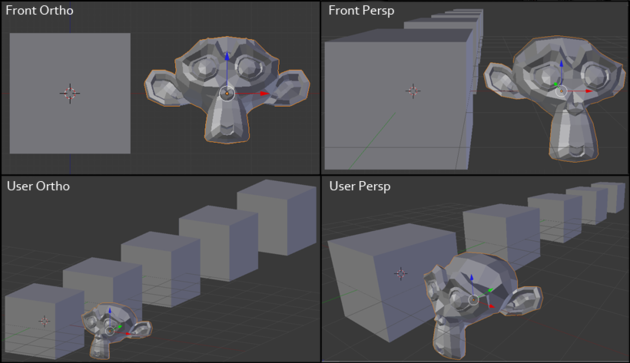
\includegraphics[width=\linewidth]{semana2/projections.png}
\caption{Proyección ortogonal y perspectiva.}
\end{wrapfigure}
Es la forma natural en que el ojo humano percibe una escena, en la proyección perspectiva los objetos distantes se ven mas pequeños que los objetos cercanos dando profundidad a distintos objetos en una escena. Este tipo de proyección es utilizada usualmente en juegos 3D.
\subsubsection{Ortogonal}
En una proyección perspectiva un objeto lejano es mas pequeño que un objeto cercano, en proyección ortogonal se ignora este efecto, eliminando la profundidad de escena. Este tipo de perspectiva es utilizada en muchos juegos 2D.
\subsection{Field Of View (FoV) o Campo de Vista}
Es el ancho del angulo de vista de la cámara, indica la extension de lo puede ver la cámara en cualquier momento, usualmente se mide en ángulos, este angulo puede ser el field of view vertical o el field of view horizontal dependiendo del framework, biblioteca o motor de juego usado (ver \ref{fig:camera}) \cite{feng_fovy}.
\subsection{Clipping Planes o Planos de Clipping}
En computación se manejan términos discretos por lo tanto una cámara no puede ver hacia el infinito, para esto están el far y near clipping planes los cuales indican donde termina el renderizado de escena y donde empieza según la posición de la cámara respectivamente (ver \ref{fig:frustum} y \ref{fig:camera}).
\subsubsection{Near Clipping Plane o Plano de Clipping Cercano}
Es donde empieza a dibujarse los objetos de escena en display, los objetos antes de este punto son ignorados por el motor gráfico.
\subsubsection{Far Clipping Plane o Plano de Clipping Lejano}
Es donde termina de dibujarse los objetos de escena en display, los objetos mas lejanos a este punto son ignorados por el motor gráfico.
\begin{figure}[H]
\centering
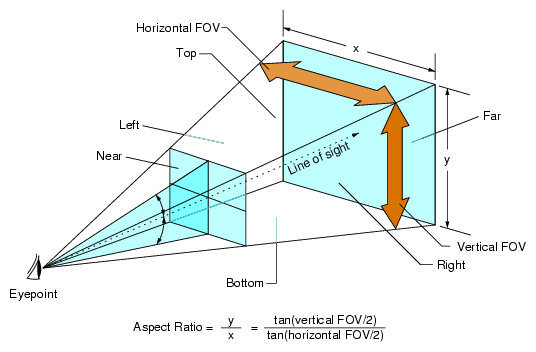
\includegraphics[width=0.9\linewidth]{semana2/camera.png} 
\caption{Parametros de una Camara Virtual}
\label{fig:camera}
\end{figure}
\newpage
\section{Tipos de Sistemas de Cámara en Vídeo Juegos}
Existen principalmente tres tipos de sistemas de cámara en vídeo juegos. En un sistema \emph{fixed} la cámara no cambia sus parámetros originales, un sistema \emph{tracking} sigue algún objeto en juego, y un sistema \emph{interactive} la cámara es parcialmente autónoma y cambia sus parámetros según distintas situaciones. Para implementar distintos sistemas de cámara los desarrolladores de vídeo juegos usan técnicas como programación con restricciones o inteligencia artificial. 
\subsection{Estáticas (\emph{Fixed})}
\begin{wrapfigure}[9]{l}{0.4\linewidth}
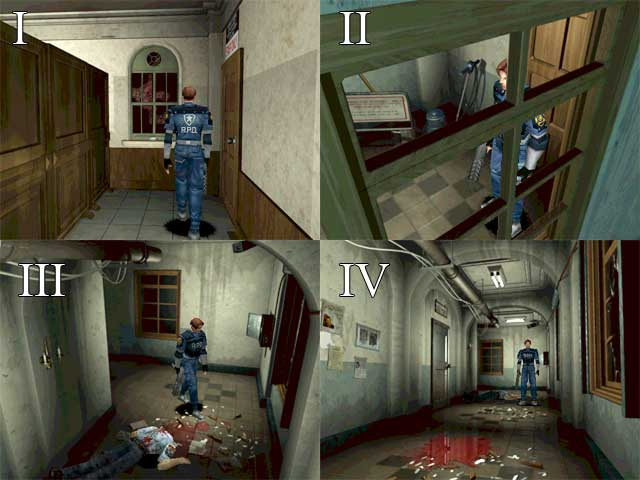
\includegraphics[width=\linewidth]{semana2/resident_evil_camerawork.jpg} 
\caption{Ejemplo de cámaras estáticas en \emph{Resident Evil 2} \cite{fixed_camera} \cite{residentevil2}.}
\end{wrapfigure}
En este tipo de cámara las propiedades de la cámara como su posición, orientación y campo visual (\emph{field of view}) son colocadas durante el desarrollo del juego y estas no cambian durante el \emph{gameplay}. Algunos ejemplos de juegos con este tipo de camara son los primeros Resident Evil, y Alone In The Dark, usualmente es utilizada para crear tension \cite{res5_review}\cite{fixed_camera}.
\subsection{Seguidoras (\emph{Tracking})}
Este tipo de cámara sigue a algún objeto en el juego usualmente el personaje principal u otro objeto de considerable importancia. Este sistema presenta varios problemas sobretodo en ambientes tridimensionales y tercera persona donde la cámara podría quedar detrás de una objeto que ocluye totalmente la vista o no deja ver algún objeto de interés al jugador \cite{fund_gamedesign}. Su uso es muy común en los primeros juegos 3D en tercera persona como \emph{Crash Bandicoot} \cite{crashbandicoot} o \emph{Tomb Raider} \cite[p.~39]{bobbatesgamedesign}, los juegos primera persona también utilizan una cámara seguidora, a diferencia de en tercera persona donde la cámara esta detrás del personaje en un juego primera persona la cámara esta como visión del personaje principal, en los juegos 2D esta cámara esta presente en todos los juegos tipo side-scroller.
\newpage
\subsection{Interactivas (\emph{Interactive})}
\begin{wrapfigure}[11]{r}{0.4\linewidth}
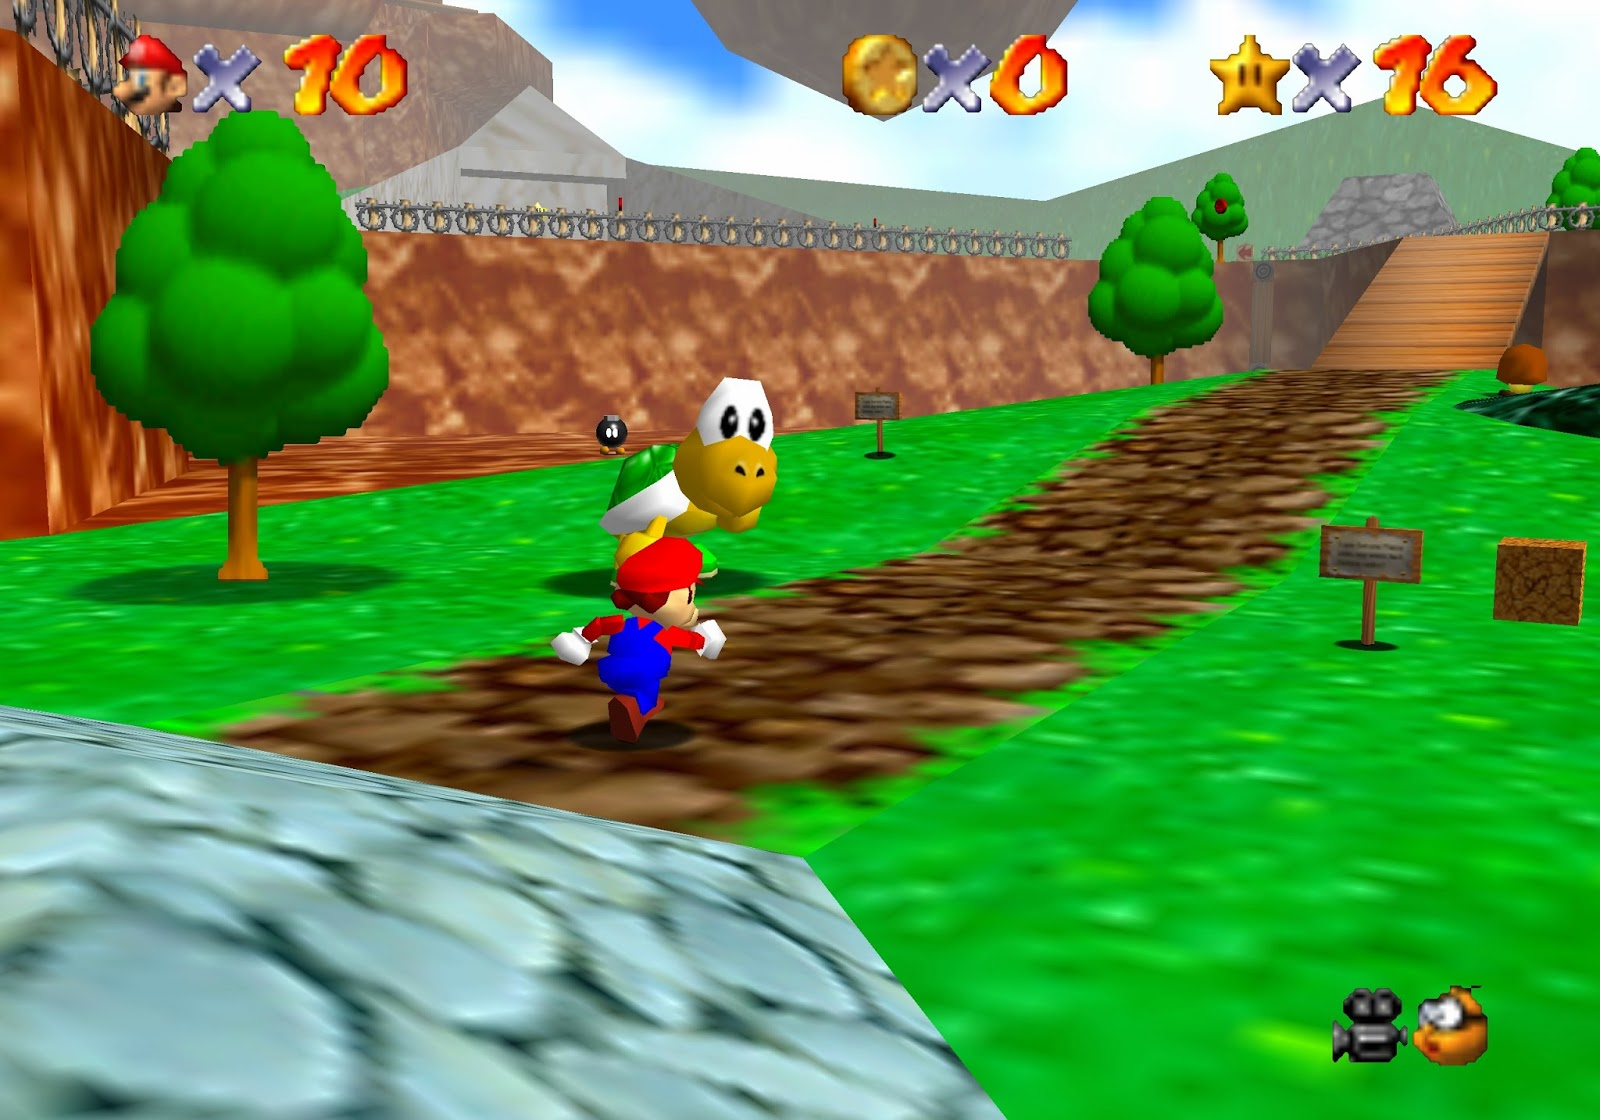
\includegraphics[width=\linewidth]{semana2/supermario64.jpg} 
\caption{En \emph{Super Mario 64} la cámara rota de forma inteligente para mostrar el camino \cite{supermario64}.}
\end{wrapfigure}
Las cámaras interactivas son cámaras que cambian su posición, campo visual u orientación según distintas situaciones, lugares o intereses del juego y sus desarrolladores, usualmente estas cámaras poseen alguna forma de inteligencia artificial. En su mayoría las cámaras interactivas son cámaras tracking mejoradas, estas siguen al personaje como lo hace una cámara tracking pero su posición y orientación puede cambiar si estas se ven obstruidas por algún objeto o cambian sus parámetros para mostrar objetos de interés claramente evitando de esta forma las desventajas principales de una cámara tracking. Algunos ejemplos de juegos con este tipo de camara son \emph{Super Mario 64}, \emph{Super Mario Sunshine}, \emph{The Legend of Zelda: The Wind Waker.}
\section{Actividad}
\begin{itemize}
\item Durante esta actividad se creara la base del proyecto y se implementara inicialmente la cámara según el diseño de su juego. Los objetivos de la actividad son:
\begin{enumerate}
  \item Crear una pequeña escena con \emph{placeholders} \footnote{Un \emph{placeholder} no es mas que un procurador de un objeto, de manera que el \emph{placeholder} es remplazado en un futuro por el objeto real.}.
  \item Implementar la cámara principal de juego según el diseño del juego.
  \item Debe crear una estructura de datos (ejemplo una clase) que defina a los actores principales en su mundo de juego, incluyendo el jugador principal. Esto depende directamente del diseño del juego.
  \item Debe asociar esta estructura a un placeholder que representa cada actor, incluyendo el jugador principal.
  \item Asocie en la lógica de juego (esto se realiza usualmente a través de scripts u otro medio que provea las herramientas que eligió) un comportamiento a uno de los actores en escena de manera que esta accion se pueda observar a través de la cámara (ejemplo moverse constantemente)
\end{enumerate}
\end{itemize}